% Copyright 2007 by Till Tantau
%
% This file may be distributed and/or modified
%
% 1. under the LaTeX Project Public License and/or
% 2. under the GNU Public License.
%
% See the file doc/licenses/LICENSE for more details.


\lecture[23]{The $F$ test}{lecture-text}

\subtitle{and two-way ANOVA}

\date{21 November 2013}

% 427-436, 449-456

\begin{document}

\begin{frame}
  \maketitle
\end{frame}



\begin{frame}{Last time}
  \begin{enumerate}
      \item Goal: test for homogeneity in means among multiple ($>2$) groups of independent samples.
      \item Tool: comparison of 
      \item how much variation there is within groups (around the group means)
      \item and how much variation there is between group means;
      \item quantified by the decomposition of the total sum-of-squares into ``within'' and ``between'' components.
          \[ 
       \SS(\text{total})  = \SS(\text{within}) + \SS(\text{between})  
   \]
  \end{enumerate}

  Equations:
    \begin{align*}
        \SS(\text{total}) &= \sum_{ij} (y_{ij} - \bar {\bar y} )^2 \\
      \df(\text{total}) &= n_\cdot - 1 \\
      \SS(\text{within}) &= \sum_{i} (n_i-1) s_i^2 = \sum_{ij} (y_{ij}-\bar y_i)^2 \\
      \df(\text{within}) &= n_\cdot - I \\
      \SS(\text{between}) &= \sum_{i} n_i (\bar y_i - \bar{\bar y_i})^2 \\
      \df(\text{between}) &= I - 1 \\
    \end{align*}
    and $\MS = \SS / \df$.
\end{frame}


%%%%%%
\begin{frame}{Example}

    Weight gain of lambs on three diets:
    \begin{center}
        \begin{tabular}{cccc}
            & Diet 1 & Diet 2 & Diet 3 \\
            & 8 & 9 & 15 \\
            & 16 & 16 & 10 \\
            & 9 & 21 & 17 \\
            &  & 11 & 6 \\
            &  & 18 &  \\
            \hline
            $n_i$ & 3 & 5 & 4 \\
            $\bar y_i$ & 11 & 15 & 12 \\
            $s_i$ & 4.359 & 4.950 & 4.967 \\
        \end{tabular}
    \end{center}

    \vspace{2em}

    Summarized:
    \begin{center}
        \begin{tabular}{cccc}
            & df & $\SS$ & $\MS$ \\
            between diets & 2 & 36 & 18 \\
            within diets & 9 & 210 & 23.33 \\
            \hline
            total & 11 & 246 & \\
        \end{tabular}
    \end{center}

\end{frame}

\begin{frame}\frametitle<presentation>{Outline}
  \tableofcontents
\end{frame}

\section{The ANOVA model}

%%%%%%
\begin{frame}{The ANOVA model}

    It is useful to think of ANOVA in terms of the following model:
    \[
        y_{ij} = \mu_i + \epsilon_{ij} ,
    \]
    where $\mu_i$ is the population mean of the $i^\mathrm{th}$ group, \\
    and the $\epsilon_{ij}$ are independent noise terms.

    \vspace{2em}

    The \structure{null hypothesis} is that
    \[ \mu_1 = \mu_2 = \cdots = \mu_I .\]


    \vspace{2em}

    A further condition is that the variance of the noise terms doesn't vary by group.

\end{frame}


%%%%%%
\begin{frame}{Relation to sum-of-squares}
    Write instead
    \[
        y_{ij} = \only<1>{\mu_i} \only<2>{\mu + (\mu_i - \mu)} \only<3->{\mu + \tau_i} + \epsilon_{ij} .
    \]
    We might estimate the various terms like so:
    \begin{align*}
        \hat \mu &= \bar{\bar y} \\
        \hat \mu_i &= \bar y_i \\
        \hat \tau_i &= \bar y_i - \bar{\bar y} \\
        \hat \epsilon_{ij} &= y_{ij} - \bar y_i .
    \end{align*}

    \vspace{2em}

    Then,
    \begin{align*}
        \SS(\text{between}) &= \sum_{i} n_i \hat \tau_i^2 \\
        \SS(\text{within}) &= \sum_{ij} \hat \epsilon_{ij}^2 .
    \end{align*}

\end{frame}

\section{The $F$ test}

%%%%%%
\begin{frame}{The $F$ statistic}

    The \structure{test statistic} we use is the ratio of mean squares within to mean squares between:
    \[
        F_s = \frac{ \MS(\text{within}) }{ \MS(\text{between}) } .
    \]


    \vspace{2em}

    The distribution of $F_s$ under the null hypothesis,  \\
    assuming that the sampling distributions of the group means are Normal, \\
    is called the \alert{$F$ distribution}, \\
    and \structure{depends on} two parameters: \\
    the degrees of freedom of the numerator and denominator.


\end{frame}


%%%%%%
\begin{frame}{Example of $F$ test}

    Weight gain of lambs on three diets
    \begin{center}
        \begin{tabular}{cccc}
            & diet 1 & diet 2 & diet 3 \\
            \hline
            $n_i$ & 3 & 5 & 4 \\
            $\bar y_i$ & 11 & 15 & 12 \\
            $s_i$ & 4.359 & 4.950 & 4.967 \\
        \end{tabular}
    \end{center}

    \pause

    \begin{center}
        \begin{tabular}{cccc}
            & df & $\SS$ & $\MS$ \\
            between diets & 2 & 36 & 18 \\
            within diets & 9 & 210 & 23.33 \\
            \hline
            total & 11 & 246 & \\
        \end{tabular}
    \end{center}


    \vspace{2em}

    With $df = (2,9)$ and
    \[ F_s = \frac{ 23.33 }{ 18 } = 0.77 , \]
    we find that $P > 0.20$.


    \vspace{2em}

    \pause
    There is not good evidence that diet affects the weight gain of lambs.


\end{frame}




\section{Conditions for the $F$ test}


%%%%%%
\begin{frame}{Conditions}

    For ANOVA to be sensible, and the $F$ test to be applicable, the following should be reasonable:
    \begin{enumerate}
        \item Each group of observations is a random sample from some population.
        \item The samples are independent of each other.
        \item The population distributions have equal standard deviations.
    \end{enumerate}

    \vspace{2em}

    In the language of the ANOVA model
    \[
        y_{ij} = \mu_i + \epsilon_{ij} ,
    \]
    the SD of the $\epsilon_{ij}$ should be the same across groups.


\end{frame}


%%%%%%
\begin{frame}{Checking the conditions}

    We don't observe the true group means $\mu_i$,
    but we have estimates:
    \[
        y_{ij} = \hat \mu_i + \hat \epsilon_{ij} ,
    \]
    so we can check the conditions by looking at the $\hat \epsilon_{ij}$.


    \pause
    \vspace{2em}

    Weight gain of lambs on three diets
    \begin{center}
        \begin{tabular}{cccc}
            & diet 1 & diet 2 & diet 3 \\
            \hline
            $n_i$ & 3 & 5 & 4 \\
            $\bar y_i$ & 11 & 15 & 12 \\
            \textbf{$s_i$} & \textbf{4.359} & \textbf{4.950} & \textbf{4.967} \\
        \end{tabular}
    \end{center}

\end{frame}


%%%%%%
\begin{frame}{Example}

    \begin{center}
\begin{tabular}{rrrrrr}
  \hline
  a & b & c & d & e \\ 
  \hline
  $n_i$ & 12.00 & 15.00 & 16.00 & 16.00 & 21.00 \\ 
  $\bar y_i$ & 1.04 & 1.70 & 2.41 & 2.93 & 0.09 \\ 
  $s_i$ & 2.72 & 17.62 & 3.73 & 9.85 & 0.38 \\ 
   \hline
\end{tabular}
    \end{center}

    \vspace{2em}

    \begin{center}
        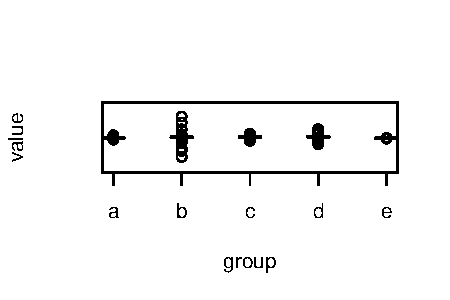
\includegraphics{ex23-1.pdf}
    \end{center}
\end{frame}

\section{Two-way ANOVA}


%%%%%%
\begin{frame}{``Factorial'' design}

    Often experiments want to examine the combined effects of several ``factors''\\
    in all their possible combinations. \\

    \vspace{2em}

    We can then ask how each factor affects the outcome on its own,\\
    and whether the effect of one factor depends on the other factor.

    \vspace{2em}


    \structure{Examples:}
    \begin{itemize}
        \item (blood pressure) :  (blood pressure medication) $\times$ (age)
        \item (beak size) : (sex) $\times$ (island)
        \item (plant growth rate) : (water) $\times$ (sunlight)
    \end{itemize}


\end{frame}

%%%%%%
\begin{frame}{Example: beak size}

    Beak size of finches in different islands:

\begin{tabular}{ccccccccccc}
    &   a & a & b & b & c & c & d & d & e & e \\
    &   F & M & F & M & F & M & F & M & F & M \\
    &     \hline
    & 10.10  &  10.66  & 11.86  &  14.67  &  10.07  & 12.95  &  11.51  &  14.60  &   12.74  & 14.33  \\
    & 9.32   &  13.31  & 14.14  &  14.60  &  10.34  & 11.39  &  13.15  &  13.88  &   13.83  & 16.18  \\
    & 8.42   &  11.88  & 10.72  &  13.97  &  8.42   & 10.86  &  12.93  &  12.48  &   12.91  & 16.42  \\
    & 7.72   &  9.88   & 13.11  &  12.55  &  8.93   & 11.09  &  13.44  &  13.58  &   13.12  & \\
    & 10.04  &  10.85  & 10.14  &  12.60  &  10.20  & 10.95  &  12.91  &  12.76  &          & \\
    & 10.24  &  11.70  & 11.20  &         &   10.93  & 9.39   &  13.08  &  14.51  &          & \\
    & 10.32  &  10.94  & 13.68  &         &   10.29  &        &   12.49  &  14.55  &          & \\
    &        &   9.72   & 12.30  &         &   11.34  &        &   13.19  &  14.81  &          & \\
    &        &   11.03  & 11.12  &         &          &         &   12.54  &  13.20  &          & \\
    &        &   10.87  & 13.24  &         &          &         &   11.29  &  13.83  &          & \\
    &        &   9.55   & 11.99  &         &          &         &   13.45  &  15.05  &          & \\
    &        &          &  10.57  &         &          &         &   11.61  &         &           & \\
    &        &          &         &          &          &         &   14.43  &         &           & \\
   \hline
   $n_i$ &   7 & 11 & 12 & 5 & 8 & 6 & 13 & 11 & 4 & 3 \\
   mean & 9.45 & 10.94 & 12.00 & 13.67 & 10.06 & 11.10 & 12.76 & 13.93 & 13.14 & 15.64 \\
   SD & 1.01 & 1.08 & 1.30 & 1.04 & 0.96 & 1.14 & 0.88 & 0.85 & 0.48 & 1.14 \\
\end{tabular}

\end{frame}

%%%%%%
\begin{frame}{Example: beak size}

    Beak size of finches in different islands:
    \begin{center}
        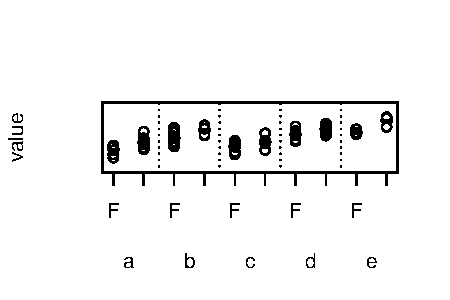
\includegraphics{ex23-beaks.pdf}
    \end{center}

    \vspace{2em}

    \begin{center}
        \begin{tabular}

        \end{tabular}
    \end{center}

\end{frame}

% two way ANOVA
%   intro additive example
%   extend model
%   intro interaction example
%   extend model
% partition of sum-squares
%   nested F test
%   summary
% (relation to t test and to chi-squared) ??


Or, Sticklebacks (has plot): http://www.plosone.org/article/info%3Adoi%2F10.1371%2Fjournal.pone.0059644

From http://www.sciencemag.org.libproxy.usc.edu/content/296/5568/707.full:

The first samples in 1973 (221 G. fortis and 72 G. scandens) were compared by ANOVAs with the last samples in 2001 (114 G. fortis and 35 G. scandens). The data were trimmed to 2.5 SD on either side of the mean by removing one to three individuals from the samples of each species. This corrected for skewness and unequal variances. Sex was included in two-factor ANOVAs because males are generally larger than females. Mean body size was significantly smaller in G. fortis (F 1,132 = 7.773, P = 0.0061) and in G. scandens (F 1,50 = 11.272, P < 0.0001) in 2001 than in 1973. There was a significant effect of sex in each species (P < 0.002) but no sex-by-year interaction (P > 0.1). Mean beak size did not differ between years in either G. fortis (F 1,166 = 0.004, P = 0.9480) or G. scandens (F 1,50 = 3.108, P= 0.0840); sex effects were significant in both species (P< 0.007), but there were no sex-by-year interactions (P> 0.1). Beak shape differed between years in both species. For G. scandens there was a strong year effect (F 1,72 = 17.168, P < 0.0001), a weak sex effect (F 1,72 = 5.943, P = 0.0172), and no interaction. The G. fortis sexes do not differ in beak shape (P = 0.9715), and therefore a one-factor ANOVA was performed with adult males, females, and birds of unknown sex. It demonstrated a strong difference between years (F 1,287 = 30.246, P < 0.0001). 

\section{Was ist Syntax?}

\begin{frame}{Die zwei Hauptbegriffe der heutigen Vorlesung.}
  \begin{block}{Grobe Definition (Syntax)}
    Unter einer \alert{Syntax} verstehen wir \alert{Regeln}, nach denen
    Texte \alert{strukturiert} werden d�rfen. 
  \end{block}
  \begin{block}{Grobe Definition (Semantik)}
    Unter einer \alert{Semantik} verstehen wir die Zuordnung von
    \alert{Bedeutung} zu Text.
  \end{block}
\end{frame}


\subsection[Syntax \protect\\ nat�rlicher Sprachen]{Syntax nat�rlicher Sprachen}

\begin{frame}{Beobachtungen zu einem �gyptischen Text.}
  \includegraphicscopyright[width=6cm]{beamerexample-lecture-pic3.jpg}
  {Copyright by Guillaume Blanchard, GNU Free Documentation License, Low Resultion}

  \begin{block}{Beobachtungen}
    \begin{itemize}
    \item Wir haben keine Ahnung, was der Text bedeutet.
    \item Es gibt aber \alert{Regeln}, die offenbar eingehalten wurden,
      wie �Hieroglyphen stehen in Zeilen�.
    \item Solche Regeln sind \alert{syntaktische Regeln} -- man kann sie
      �berpr�fen, ohne den Inhalt zu verstehen.
    \end{itemize}
  \end{block}
\end{frame}


% . . . 

\section<article>{Summary}
\section<presentation>*{Summary}

\begin{frame}{Summary}
  \begin{enumerate}
  \item Ein \alert{Wort} ist eine Folge von Symbolen aus einem
    \alert{Alphabet}. 
  \item Eine \alert{Syntax} besteht aus Regeln, nach denen
    Worte (Texte) gebaut werden d�rfen.
  \item Eine \alert{Semantik} legt fest, was Worte \alert{bedeuten}.
  \item Eine \alert{formale Sprache} ist eine Menge von Worten
    �ber einem Alphabet.
  \end{enumerate}
\end{frame}

% homework
\begin{frame}{Homework}
  \begin{center}

  % 7.4.2

  \vspace{2em}

  % 7.4.8

  \vspace{2em}

  % 7.5.1

  \end{center}
\end{frame}


\end{document}





